\documentclass[11pt]{aghdpl}
% \documentclass[en,11pt]{aghdpl}  % praca w języku angielskim

% Lista wszystkich języków stanowiących języki pozycji bibliograficznych użytych w pracy.
% (Zgodnie z zasadami tworzenia bibliografii każda pozycja powinna zostać utworzona zgodnie z zasadami języka, w którym dana publikacja została napisana.)
\usepackage[english,polish]{babel}

% Użyj polskiego łamania wyrazów (zamiast domyślnego angielskiego).
\usepackage{polski}

\usepackage[utf8]{inputenc}

% dodatkowe pakiety

\usepackage{mathtools}
\usepackage{amsfonts}
\usepackage{amsmath}
\usepackage{amsthm}

% --- < bibliografia > ---

\usepackage[
style=numeric,
sorting=none,
%
% Zastosuj styl wpisu bibliograficznego właściwy językowi publikacji.
language=autobib,
autolang=other,
% Zapisuj datę dostępu do strony WWW w formacie RRRR-MM-DD.
urldate=iso8601,
% Nie dodawaj numerów stron, na których występuje cytowanie.
backref=false,
% Podawaj ISBN.
isbn=true,
% Nie podawaj URL-i, o ile nie jest to konieczne.
url=false,
%
% Ustawienia związane z polskimi normami dla bibliografii.
maxbibnames=3,
% Jeżeli używamy BibTeXa:
backend=bibtex
]{biblatex}

\usepackage{csquotes}
% Ponieważ `csquotes` nie posiada polskiego stylu, można skorzystać z mocno zbliżonego stylu chorwackiego.
\DeclareQuoteAlias{croatian}{polish}

\addbibresource{bibliografia.bib}

% Nie wyświetlaj wybranych pól.
%\AtEveryBibitem{\clearfield{note}}


% ------------------------
% --- < listingi > ---

% Użyj czcionki kroju Courier.
\usepackage{courier}

\usepackage{listings}
\lstloadlanguages{TeX}

\lstset{
        literate={ą}{{\k{a}}}1
           {ć}{{\'c}}1
           {ę}{{\k{e}}}1
           {ó}{{\'o}}1
           {ń}{{\'n}}1
           {ł}{{\l{}}}1
           {ś}{{\'s}}1
           {ź}{{\'z}}1
           {ż}{{\.z}}1
           {Ą}{{\k{A}}}1
           {Ć}{{\'C}}1
           {Ę}{{\k{E}}}1
           {Ó}{{\'O}}1
           {Ń}{{\'N}}1
           {Ł}{{\L{}}}1
           {Ś}{{\'S}}1
           {Ź}{{\'Z}}1
           {Ż}{{\.Z}}1,
        basicstyle=\footnotesize\ttfamily,
}

% ------------------------

\AtBeginDocument{
        \renewcommand{\tablename}{Tabela}
        \renewcommand{\figurename}{Rys.}
}

% ------------------------
% --- < tabele > ---

\usepackage{array}
\usepackage{tabularx}
\usepackage{multirow}
\usepackage{booktabs}
\usepackage{makecell}
\usepackage{tikz}
\usepackage[flushleft]{threeparttable}

% defines the X column to use m (\parbox[c]) instead of p (`parbox[t]`)
\newcolumntype{C}[1]{>{\hsize=#1\hsize\centering\arraybackslash}X}


%---------------------------------------------------------------------------

\author{Radosław Sajdak}
\shortauthor{R. Sajdak}

%\titlePL{Przygotowanie bardzo długiej i pasjonującej pracy dyplomowej w~systemie~\LaTeX}
%\titleEN{Preparation of a very long and fascinating bachelor or master thesis in \LaTeX}

\titlePL{Opracowanie urządzenia wykrywającego wypadek rowerowy z powiadamianiem GSM}
\titleEN{Development of a bicycle accident detection device with GSM notification}


\shorttitlePL{Opracowanie urządzenia wykrywającego wypadek rowerowy} % skrócona wersja tytułu jeśli jest bardzo długi
\shorttitleEN{Development of a bicycle accident detection device}

\thesistype{Praca dyplomowa inżynierska}
%\thesistype{Master of Science Thesis}

\supervisor{dr inż. Łukasz Krzak}
%\supervisor{Marcin Szpyrka PhD, DSc}

\degreeprogramme{Elektronika i Telekomunikacja}
%\degreeprogramme{Computer Science}

\date{2022}

\department{Katedra Elektroniki}
%\department{Department of Applied Computer Science}

\faculty{Wydział Informatyki, Elektroniki,\protect\\[-1mm] i Telekomunikacji}
%\faculty{Faculty of Electrical Engineering, Automatics, Computer Science and Biomedical Engineering}

\acknowledgements{Serdecznie dziękuję \dots tu ciąg dalszych podziękowań np. dla promotora, żony, sąsiada itp.}


\setlength{\cftsecnumwidth}{10mm}

%---------------------------------------------------------------------------
\setcounter{secnumdepth}{4}
\brokenpenalty=10000\relax

\begin{document}

\titlepages

% Ponowne zdefiniowanie stylu `plain`, aby usunąć numer strony z pierwszej strony spisu treści i poszczególnych rozdziałów.
\fancypagestyle{plain}
{
        % Usuń nagłówek i stopkę
        \fancyhf{}
        % Usuń linie.
        \renewcommand{\headrulewidth}{0pt}
        \renewcommand{\footrulewidth}{0pt}
}

\setcounter{tocdepth}{2}
\tableofcontents
\clearpage

%\chapter{Przykłady elementów pracy dyplomowej}

\section{Liczba}

Pakiet \texttt{siunitx} zadba o to, by liczba została poprawnie sformatowana: \\
\begin{center}
	\num{1234567890.0987654321}
\end{center}


\section{Rysunek}

Pakiet \texttt{subcaption} pozwala na umieszczanie w podpisie rysunku odnośników do ,,podilustracji'': \\

\begin{figure}[h]
	\centering
	\begin{subfigure}{0.35\textwidth}
		\centering
		\framebox[2.0\width]{A}
		\subcaption{\label{subfigure_a}}
	\end{subfigure}
	\begin{subfigure}{0.35\textwidth}
		\centering
		\framebox[2.0\width]{B}
		\subcaption{\label{subfigure_b}}
	\end{subfigure}
	
	\caption{\label{fig:subcaption_example}Przykład użycia \texttt{\textbackslash subcaption}: \protect\subref{subfigure_a} litera A, \protect\subref{subfigure_b} litera B.}
\end{figure}

\section{Tabela}

Pakiet \texttt{threeparttable} umożliwia dodanie do tabeli adnotacji: \\

\begin{table}[h]
	\centering
	
	\begin{threeparttable}
		\caption{Przykład tabeli}
		\label{tab:table_example}
		
		\begin{tabularx}{0.6\textwidth}{C{1}}
			\toprule
			\thead{Nagłówek\tnote{a}} \\
			\midrule
			Tekst 1 \\
			Tekst 2 \\
			\bottomrule
		\end{tabularx}
		
		\begin{tablenotes}
			\footnotesize
			\item[a] Jakiś komentarz\textellipsis
		\end{tablenotes}
		
	\end{threeparttable}
\end{table}

\section{Wzory matematyczne}

Czasem zachodzi potrzeba wytłumaczenia znaczenia symboli użytych w równaniu. Można to zrobić z użyciem zdefiniowanego na potrzeby niniejszej klasy środowiska \texttt{eqwhere}.

\begin{equation}
E = mc^2
\end{equation}
gdzie
\begin{eqwhere}[2cm]
	\item[$m$] masa
	\item[$c$] prędkość światła w próżni
\end{eqwhere}

Odległość półpauzy od lewego marginesu należy dobrać pod kątem najdłuższego symbolu (bądź listy symboli) poprzez odpowiednie ustawienie parametru tego środowiska (domyślnie: 2 cm).

\chapter{Wstęp}
\label{cha:wstep}

Obecny rozwój mikroprocesorów, pozwala na tworzenie coraz bardziej złożonych urządzeń. Rozwój układów o niskim zużyciu energii, popycha elektronikę w kierunku małych, wielofunkcyjnych urządzeń. Połączenie tych dwóch procesów pozwala na stworzenie elastycznych urządzeń, których zastosowanie może zmieniać się jedynie dzięki oprogramowaniu.

%---------------------------------------------------------------------------

\section{Cele pracy}
\label{sec:celePracy}

Rowerzyści górscy, podczas samotnych wypraw rowerowych, wielokrotnie zastanawiają się, co w sytuacji, gdy ulegną wypadkowi podczas samotnej wyprawy?
Jak długo nikt nie wezwie pomocy? W ten sposób, powstał pomysł stworzenia urządzenia asystującego.
\newline
Celem pracy było stworzenie innowacyjnego urządzenia wykrywającego upadek na rowerze. Urządzenie miało być przymocowane do ramy roweru. Urządzenie, informację o wypadku wysyła przy użyciu modemu LTE-M opartego o interfejs szeregowy UART. Za lokalizowanie urządzenia, odpowiadać będzie moduł GPS oparty o magistralę $I^{2}C$. Całość, sterowana będzie przy użyciu mikrokontrolera.

\section{Analiza wymagań technicznych i dobór komponentów}
\label{sec:technical_analysis}
Docelowo, urządzenie miało zwiększać bezpieczeństwo podczas wypraw rowerowych. Musiało więc być bardzo energooszczędne. Minimalne wymaganie, to 24 godziny pracy na jednym ładowaniu baterii. Jednocześnie, nie może być zbyt duże, aby w łatwy sposób można było zamontować je na rowerze. Pobierana lokalizacja, miała mieć dokładność około 100m. Jest to dokładność wystarczająca, aby zobaczyć ranną osobę, leżący rower, lub usłyszeć wołanie o pomoc. Ważnym było, aby urządzenie, było w pełni niezależne od innych układów, jak np. telefon.
\newline
Planując pracę, zdecydowano się wykorzystać trzy moduły:
\begin{itemize}
    \item Akcelerometr
    \item GPS
    \item LTE
\end{itemize}
Dodatkowo, ze względu na łatwy w użyciu stos Bluetooth, wykorzystano również Bluetooth Low Energy, celem stworzenia bezprzewodowego interfejsu sterowania urządzeniem.
\newline
Ponieważna rynku dostępnych było wiele różnych modułów, poniżej dokonano ich porównania oraz wyboru układów, najbardziej pasujących do stworzonego rozwiązania.

\subsection{Akcelerometr}
Akcelerometry to układy, mierzące przyspieszenie. Mogą dokonać pomiaru przyspieszenia statycznego (np. Ziemskiego), lub dynamicznego, działającego z sił, działających na układ. W przypadku dostępnych na rynku akcelerometrów należy pamiętać, że w stanie spoczynku wskazują one przyspieszenie około $9.81\frac{m}{s^{2}}$. Można więc było, wykorzystać ten fakt, do implementacji algorytmu.
\newline
Obecnie, większość układów to układy integrujące akcelerometr i żyroskop w jednym układzie scalonym. Coraz częściej, można też spotkać magnetometr. Dla obecnych na rynku układów, wyróżniamy dwa najważniejsze parametry:
\begin{itemize}
    \item Zakres pracy akcelerometru - określany jako $\pm X_{g}$, a więc przyspieszenie w trzech kierunkach, podane jako wielokrotność przyspieszenia Ziemskiego. Zazwyczaj, wartość ta, mieści się w przedziale od kilku, do kilkunastu g.
    \item Zakres pomiarów żyroskopu - określony jako \emph{dps (degrees per second)}. Jeśli prędkość kątowa będzie większa, niż wybrany zakres, układ ulegnie nasyceniu
\end{itemize}
Głównym wymaganiem dotyczącym akcelerometru, była jego energooszczędność. Był to jedyny układ, który działa przez cały czas. Z tego powodu, akcelerometr powinien był nie tylko zużywać mało prądu, ale również posiadać różne tryby pracy. Dodatkowym atutem, była wbudowana pamięć, pozwalająca na buforowanie danych.
\newline
Spośród dostępnych na rynku układów, wybrane zostały trzy, dostępne w trakcie tworzenia pracy.

\subsubsection{MPU-6050}
Wybrany układ, jest 3-osiowym akcelerometem i żyroskopem. Korzysta on z magistrali $I^{2}C$. Zgodnie z dokumentacją układu, w normalnym trybie pracy, można spodziewać się ok. 3.8mA prądu, pobieranego przez układ.\cite{MPU6050} Wartość tę, można zredukować do nawet 10$\mu$A, ograniczając częstotliwość próbkowania akcelerometru do 1.25Hz i wyłączając żyroskop. Ponadto, układ posiada tryb niskiego zużycia energii, pozwalający uśpić nieaktywny układ. Sam akcelerometr, pracuje w zakresie $\pm$2g, $\pm$4g, $\pm$8g oraz $\pm$16g. Dodatkowo, układ posiada tzw. Digital Motion Pocessor (DMP), czyli układ wspomagający przetwarzanie danych w kierunku wykrywania gestów. Wbudowane FIFO, pozwala na buforowanie danych. Zaletą akcelerometru, są programowalne przerwania oraz przerwanie "High-G", wyzwalane w momencie przekroczenia zdefiniowanego przyspieszenia.

\subsubsection{LSM9DS1}
Układ ten, nie różni się znacząco od MPU-6050. Zgodnie z dokumentacją, jest on dodatkowo wyposażony w magnetometr. Największą z różnic, jest pobierany przez niego prąd. W przypadku LSM9DS1, akcelerometr w trybie normalnym, pobiera około 600$\mu$A.\cite{LSM9DS1} Niestety, wykorzystanie żyroskopu, dodaje kolejne 4mA. Żyroskop, posiada tryb niskiego zużycia energii, pozwalający ograniczyć zużycie energii do 1.9mA. Tym samym, układ nie jest w stanie zejść poniżej 1.96mA, co znacząco przekraczało domniemany pobór prądu.

\subsubsection{LSM6DSOX}
Ostatni z wybranych układów, był układem producenta ST. Jest on dedykowany do rozwiązań, o niskim zużyciu energii. Według dokumentacji, jego zużycie energii to 550$\mu$A.\cite{LSM6DSOX} Wartość ta, jest kilkukrotnie niższa, niż w przypadku MPU-6050. Co więcej, układ posiada tryb LowPower, w którym zużycie energii można ograniczyć do nawet 4$\mu$A. LSM6DSOX, posiada również 9kB FIFO, po którego napełnieniu, wystawiane jest przerwanie. Dodatkową zaletą, jest szesnaście programowalnych maszyn stanów. Pozwalają one na maksymalne ograniczanie zużycia energii, dzięki możliwości wyłączenia mikrokontrolera w trybie analizy danych. LSM6DSOX, do komunikacji wykorzystuje $I^{2}C$. Pozostałe jego parametry, są zbliżone do opisywanych wcześniej.

\subsubsection{Wybór akcelerometru}
Spośród trzech dostępnych układów, wybrany został LSM6DSOX. Jak pokazuje tabela \ref{tab:accelerometer}, układy te, są stosunkowo podobne. Decydującym elementem, okazały się być maszyny stanów, wbudowane w akcelerometr. Pozwoliły one znacząco ograniczyć zużycie energii całego układu oraz przyspieszyć proces tworzenia aplikacji.

\begin{table}[h]
\centering
\begin{tabular}{|c | c | c | c|}
    \hline
     & MPU-6050 & LSM9DS1 & LSM6DSOX \\
    \hline
    FIFO & 1kB  &   128B  & 9kB \\
    \hline
    Prąd pracy  & 3.8 mA & 600 $\mu$A & 550 $\mu$A \\
    \hline
    Low Power & 10-110 $\mu$A & 1.9-3.1 mA & 4-20 $\mu$A\\
    \hline
    Zakres pracy & 2-16g & 2-16g & 2-16g\\
    \hline
\end{tabular}
\caption{Porównanie dostępnych akcelerometrów}
\label{tab:accelerometer}
\end{table}

\subsection{Mikrokontroler}
Mikrokontroler, jest mózgiem układu. z tego powodu, wybrany układ musiał być bardzo wydajny, ale Jednocześnie energooszczędny. Kolejnym z wymagań, była obsługa interfejsu I$^{2}$C oraj UART. Ponieważ wybrany akcelerometr posiada dwa piny przerwań zewnętrznych, mikrokontroler musiał być gotowy je obsłużyć.

\subsubsection{ATmega328p}
Mikrokontroler ATmega328p, to jeden z najpopularniejszych układów na rynku. Jego niska cena i łatwość użycia, pozwala budować najróżniejsze aplikacje. Układ wspiera zewnętrzny zegar o częstotliwości do 16MHz. Posiada on UART, I$^{2}$C oraz SPI, co pozwoliło rozważyć go w pracy. Dodatkowo, w dokumentacji, można znaleźć informację o dwóch przerwaniach zewnętrznych, obsługiwanych przez układ.\cite{ATMEGA328P} Dla najwyższej częstotliwości, podczas pracy układ pobiera 9-14mA. Wartość ta, może zostać ograniczona do 2.8mA w trybie czuwania. W trybie zupełnego uśpienia, mikrokontroler pobiera pomiędzy 44, a 66$\mu$A.

\subsubsection{STM32F303K8}
Układ STM32F303K8 oparty jest na rdzeniu ARM Cortex M4. Posiada on wbudowany układ czasu rzeczywistego z funkcją wybudzania z kalendarzem. 11 wbudowanych liczników, pozwala na budowanie wyjątkowo złożonych aplikacji. Mikrokontroler wyposażono w SPI, I$^{2}$C, SPI, oraz 3 UARTy. W przypadku rdzeni Cortex, każdy z pinów może być skonfigurowany jako przerwanie, co daje nam aż 60 przerwań. \cite{STM32F303K8} Układ, może być taktowany zewnętrznym zegarem o częstotliwości do 32MHz, a więc dwukrotnie większym, niż w przypadku kontrolera ATmega. STM32F303K8 pobiera (w zależności od konfiguracji) 12.9 - 34mA w trybie pracy oraz 0.93-18.57$\mu$A w trybie głębokiego uśpienia. Warto zaznaczyć, że wartości maksymalneukład osiąga, gdy wszystkie peryferia są uruchomione. W przypadku tej pracy, dążono do minimalizacji ilości działających podzespołów.

\subsubsection{nRF52840}
Mikrokontroler nRF52840 jest najmocniejszym spośród wybranych do tego porównania. Oparty na rdzeniu ARM Cortex M4, taktowany zegarem 64MHz, posiada 1MB pamięci flash oraz 256kB RAM. Wspiera on I$^{2}$C, 4x SPI, 2x UART i 3xRTC. Obsługuje też Bluetooth, co wyróżnia go na tle dwóch pozostałych układów. Mimo, że posiada on tak dużo peryferiów, jego zużycie energii w trybach głębokiego uśpienia mieści się pmiędzy 0.4uA, a 17.37uA. Są to wartości zbliżone do kontrolra STM32F303K8, opartego na tym samym rdzeniu. Pracujący układ, w zależności od konfiguracji, zużywa 2.8-6.3mA. Dodatkowo, nRF52840 posiada wbudowane PMU (Power Management Unit), które automatycznie zarządza zużywaną energią, bez ingerencji użytkownika. Zaletą, jest również bardzo obszerna dokumentacja\cite{NRF52840}, dedykowane fora wsparcia oraz powszechność stosowania tego układu w urządzeniach.

\subsubsection{Wybór mikrokontrolera}
Porównanie układów pokazało, że prosta ATmega328p znacząco odstaje od pozostałych układów. Mimo, że jest najprostszym z układów, nie mógł zostać wykorzystany w pracy, ze względu na wysokie zużycie energii. Problemem mogła okazać się również niewielka liczba liczników. W tym przypadku, najlepiej wypadł STM32F303K8. Niestety, jego wadą było wysokie zużycie energii w trakcie pracy. Z tego powodu, ostateczny wybór padł na nRF52840. Podsumowanie porównania, obrazuje poniższa tabela.\ref{tab:microcontroller}

\begin{table}[h]
    \centering
    \begin{tabular}{|c | c | c | c|}
        \hline
         & ATmega328p & STM32F303K8 & nRF52840 \\
        \hline
        FLASH & 32kB  &   64kB  & 1MB \\
        \hline
        Prąd pracy  & 9.3-14 mA & 12.9-34 mA &2.8-6.3 mA \\
        \hline
        Low Power & 40-66 $\mu$A & 0.93-18.57 $\mu$A & 0.4-17.37 $\mu$A\\
        \hline
        Liczniki & 2x8bit, 1x16bit & 1x32bit, 2x24bit, 8x16bit & 5x32bit\\
        \hline
        I$^{2}$C & \cmark & \cmark & \cmark\\
        \hline
        UART & 1 & 3 & 2\\
        \hline
        Przerwania zewnętrzne & 2 & 16 & 48\\
        \hline
        System operacyjny & Brak & Free RTOS & Zephyr RTOS\\
        \hline
    \end{tabular}
    \caption{Porównanie dostępnych mikroprocesorów}
    \label{tab:microcontroller}
    \end{table}

\subsection{Modem GSM/LTE}
Modem GSM/LTE to układ pozwalający na komunikację przez sieci komórkowe 4G lub GSM. Zastosowanie tego typu komunikacji, pozwoliło zapewnić dostęp do sieci niemal niezależnie od miejsca w którym znajdowało się urządzenie. Ponieważ procedura autentykacji do sieci jest czasochłonna i wymaga radzia, działającego z dużą mocą. Zgodnie z przewidywaniami, był jest to układ o największym zużyciu energii. Minimalnym wymaganiem dotyczącym tego układu, jest obsługa SMS. Podczas rozważań nad wyborem modemu, dodatkową zaletą była obsługa zapytań HTTP. Pozwoliła ona na przetestowanie alternatywnego podejścia do problemu powiadamiania.

\subsubsection{SIM800L}
SIM800L to jeden z najpopularniejszych układów do amatorskich rozwiązań. Jego największymi zaletami są cena i mnogość dostępnych bibliotek czy przykładów. Niestety, głównie dedykowanych do mikrokontrolera ATmega328p. Zastosowanie go z innymi układami nie jest jednak problemem, ponieważ działa on w oparciu o tak zwane komendy AT, wysyłane przez UART. Pobór prądu tego modemu, mieści się pomiędzi 150, a 450mA podczas transmisji danych. oraz 50-60$\mu$ w trybie PowerDown. Co ważne, podczas uruchamiania, układ pobiera do 2A prądu, co jest wartością bardzo dużą, w przypadku układów zasilanych bateryjnie. Niestety, układ ten działa z przestarzałymi już sieciami GSM i nie obsługuje zapytań HTTP.\cite{SIM800L}

\subsubsection{Quectel EC20 R2.1}
Jest to jeden z łatwo dostępnych na rynku układów, działających w oparciu o technologię LTE. komunikacja z nim, przebiega przy użyciu komend AT. Układ, wspiera możliwość wysyłania zapytań HTTP. Pobór prądu modemu, osiąga 300mA, jednak w tybie PowerDown, wynosi jedynie 11$\mu$A. Jest to więc wartość ponad pięciokrotnie mniejsza, niż w przypadku SIM800L. Jest to ważne, ponieważ projektowane urządzenie miało pracować większość czasu w trybie całkowitego uśpienia. W przypadku tego układu, problemem było również znalezienie pełnej dokumentacji.

\subsubsection{SKY66430}
Jest to produkt firmy Skyworks, specjalizującej się w tworzeniu półprzewodników do układów radiowych i komunikacji mobilnej. Wybrany modem, działa w technologii LTE-M, co wymagało zakup specjalnych kart SIM. Układy LTE-M, zużywają znacznie mniej energii niż układy komunikujące się przez zwykłą sieć 4G. Są też w stanie transmitować z miejsc, o bardzo słabym zasięgu. SKY66430 podczas transmisji pobiera 150-250mA prądu, a w trybie PowerDown jedynie 1$\mu$A. Wartości te, uczyniły go więc najlepszym z rozważanych układów. Dodatkowym jego atutem jest obsługa zapytań HTTP. \cite{SKY66430}

\begin{table}[h]
    \centering
    \begin{tabular}{|c | c | c | c|}
        \hline
         & SIM800L & Quectel EC20 R2.1 & SKY66430 \\
        \hline
        Prąd pracy  & 150-450 mA & 300 mA &150-250 mA \\
        \hline
        PowerDown & 50-60 $\mu$A & 11 $\mu$A & 1 $\mu$A\\
        \hline
        SMS & \cmark & \cmark & \cmark\\
        \hline
        HTTP & \xmark & \cmark & \cmark\\
        \hline
    \end{tabular}
    \caption{Porównanie dostępnych mikroprocesorów}
    \label{tab:modem}
    \end{table}

\subsubsection{Wybór modemu}
Analizując powyższe dane, nie sposób było wybrać układ inny, niż SKY66430. Jest to układ o zdecydowanie najniższym zużyciu energii. Co więcej, wspiera on zapytania HTTP, co pozwoliło na przeprowadzenie dodatkowych testów projektu.

\subsection{GPS}
GPS, czyli Global Positioning System, to system nawigacji oparty na lokalizacji satelitarnej. Jego zadaniem, jest dostarczenie użytkownikom informacji o ich położeniu. W przypadku projektowanego urządzenia, kluczowym było pozyskanie możliwie dokładnej lokalizacji. Tak jak w przypadku pozostałych komponentów, układ powinien był charkteryzować się jak najniższym zużyciem energii. Ponieważ układ ten mógł okazać się najbardziej energochłonny, dodatkowym wymaganiem była możliwość jego wyłączenia. Istotnym elementem była również dokładność określanego położenia. Jako wystarczająca, uznana została dokładność 100m.

\subsubsection{Beitian BN-220}
Jest to jeden z najtańszych układów dostępnych na rynku. Układ, komunikuje się przy użyciu interfejsu UART, przesyłając wiadomości NMEA. Są to zdania, zapisane kodem ASCII, ustandaryzowanej strukturze. Zgodnie z dokumentacją, układ pobiera około 50mA i jest zasilany napięciem 5V.\cite{BN220}

\subsubsection{Mediatek MT3339}
Kolejny układ, zasilany jest napięciem 3.3V i pobiera około 3mA prądu. Tak, jak BN-220, komunukuje się przy użyciu wiadomości NMEA, jednak korzystając z magistrali I$^{2}$C. Dodatkowo, układ ten, posiada wewnętrzny zegar czasu rzeczywistego, pozwalający na wybudzenie układu ze stanu uśpienia. Ciekawą funkcjonalnością tego modułu, jest obsługa EPO. Jest to predykcja położenia satelit, na podstawie czasu i zapisanego w pamięci pliku. Dzięki temu rozwiązaniu, można znacząco skracać czas określania lokalizacji. Dokładność urządzenia to około 3m, co jest wartością znacznie większą niż zakładana.\cite{MT3339}

\subsubsection{Mediatek MT3333}
MT3333 to układ bardzo zbliżony do wspomnianego wcześniej MT3339. Różnią się one zużyciem energii. W przypadku MT3333, pobór prądu wynosi od 5 do 19mA. Podobnie jak poprzednik, komunikuje się on przy użyciu wiadomości NMEA, przesyłanych magistralą I$^{2}$C.\cite{MT3333}

\subsubsection{Wybór modułu GPS}
Pomimo, że układ MT3339 cechuje się najmniejszym zużyciem energii oraz posiada interesujące funkcjonalności, zdecydowano się na wybór modułu Mediatek MT3333. Wynikło to bezpośrednio z faktu, że w momencie tworzenia pracy, dostępna była tylko dokumentacja do układu MT3333. Ponieważ jednak układy te są zgode ze standardem oraz korzystają z tego samego interfejsu komunikacji, możliwą byłaby podmiana układów.

\begin{table}[h]
    \centering
    \begin{tabular}{|c | c | c | c|}
        \hline
         & BN-220 & MT3339 & MT3333 \\
        \hline
        Prąd pracy  & 50 mA & 3 mA &5-19 mA \\
        \hline
        Interfejs & UART & I$^{2}$C & I$^{2}$C\\
        \hline
    \end{tabular}
    \caption{Porównanie dostępnych modułów GPS}
    \label{tab:gps}
    \end{table}


\section{Podsumowanie wyboru sprzętu}
Rozważane w sekcji \ref{sec:technical_analysis} komponenty, zostały dobrane przede wszystkim ze względu na niskie zużycie energii. Każdy z wybranych komponentów, testowany był przy użyciu płytek rozwojowych, dostępnych w sklepach. Dodatkowo, taki wybór komponentów, pozwolił skorzystać z gotowej płytki PCB, stosowanej w jednym z dostępnych na rynku urządzeń. Zmiana oprogramowania urządzenia, przy użyciu programatora J-link, pozwoliła zupełnie zmienić jego zastosowanie. Takie podejście, umożliwiło rownież stworzenie prototypu urządzenia, które rozwijane może trafić na rynek, bez kosztownego projektowania nowych płytek PCB. (rys. \ref{img:pcb})

\begin{figure}[t]
    \centering
    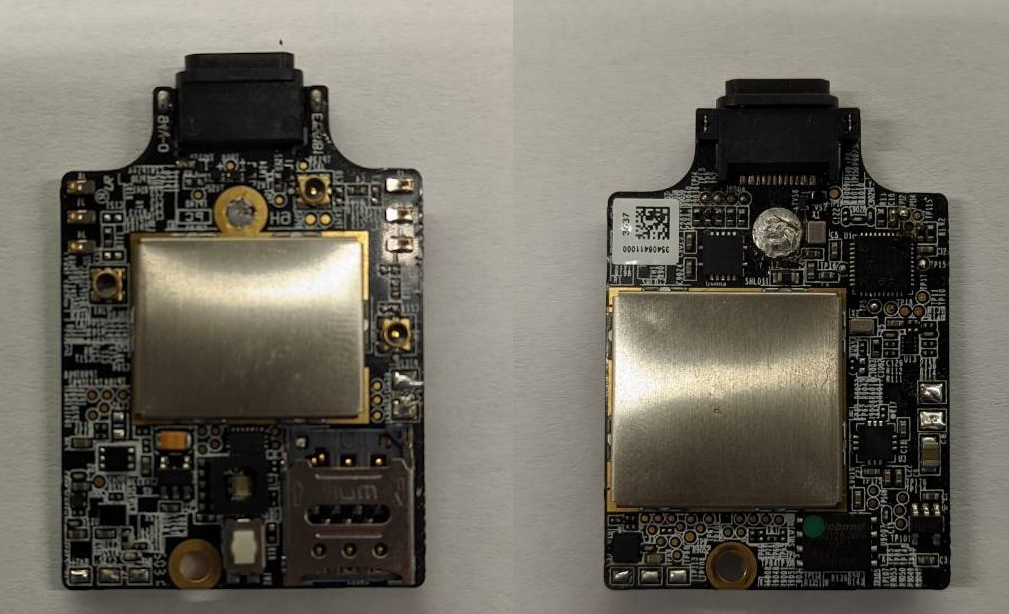
\includegraphics[width=7cm]{Graphics/PCB.png}
    \caption{Wykorzystana płytka PCB z urządzenia dostępnego na rynku}
    \label{img:pcb}
\end{figure}
\section{Podobne rozwiązania obecne na rynku}
Podobne rozwiązanie, zaproponowała firma Specialized. Inżynierowie stworzyli urządzenie o nazwie ANGI, widoczne na rysunku \ref{img:angi_img}. Jest to mały układ, wyposażony w akcelerometr i żyroskop. Komunikuje się on przy użyciu Bluetooth z ich autorską aplikacją na telefon z iOS lub Androidem. Urządzenie, zamontowane na kask, wysyła powiadomienie do aplikacji, gdy rowerzysta uderza kaskiem w przeszkodę. Rozwiązanie to, ma szereg zalet, takich jak prostota budowy i bardzo niskie zużycie energii. Jest ono jednak uzależnione od telefonu, który w przypadku wycieczek górskich, czasem wygodniej zostawić w domu.
\begin{figure}[h]
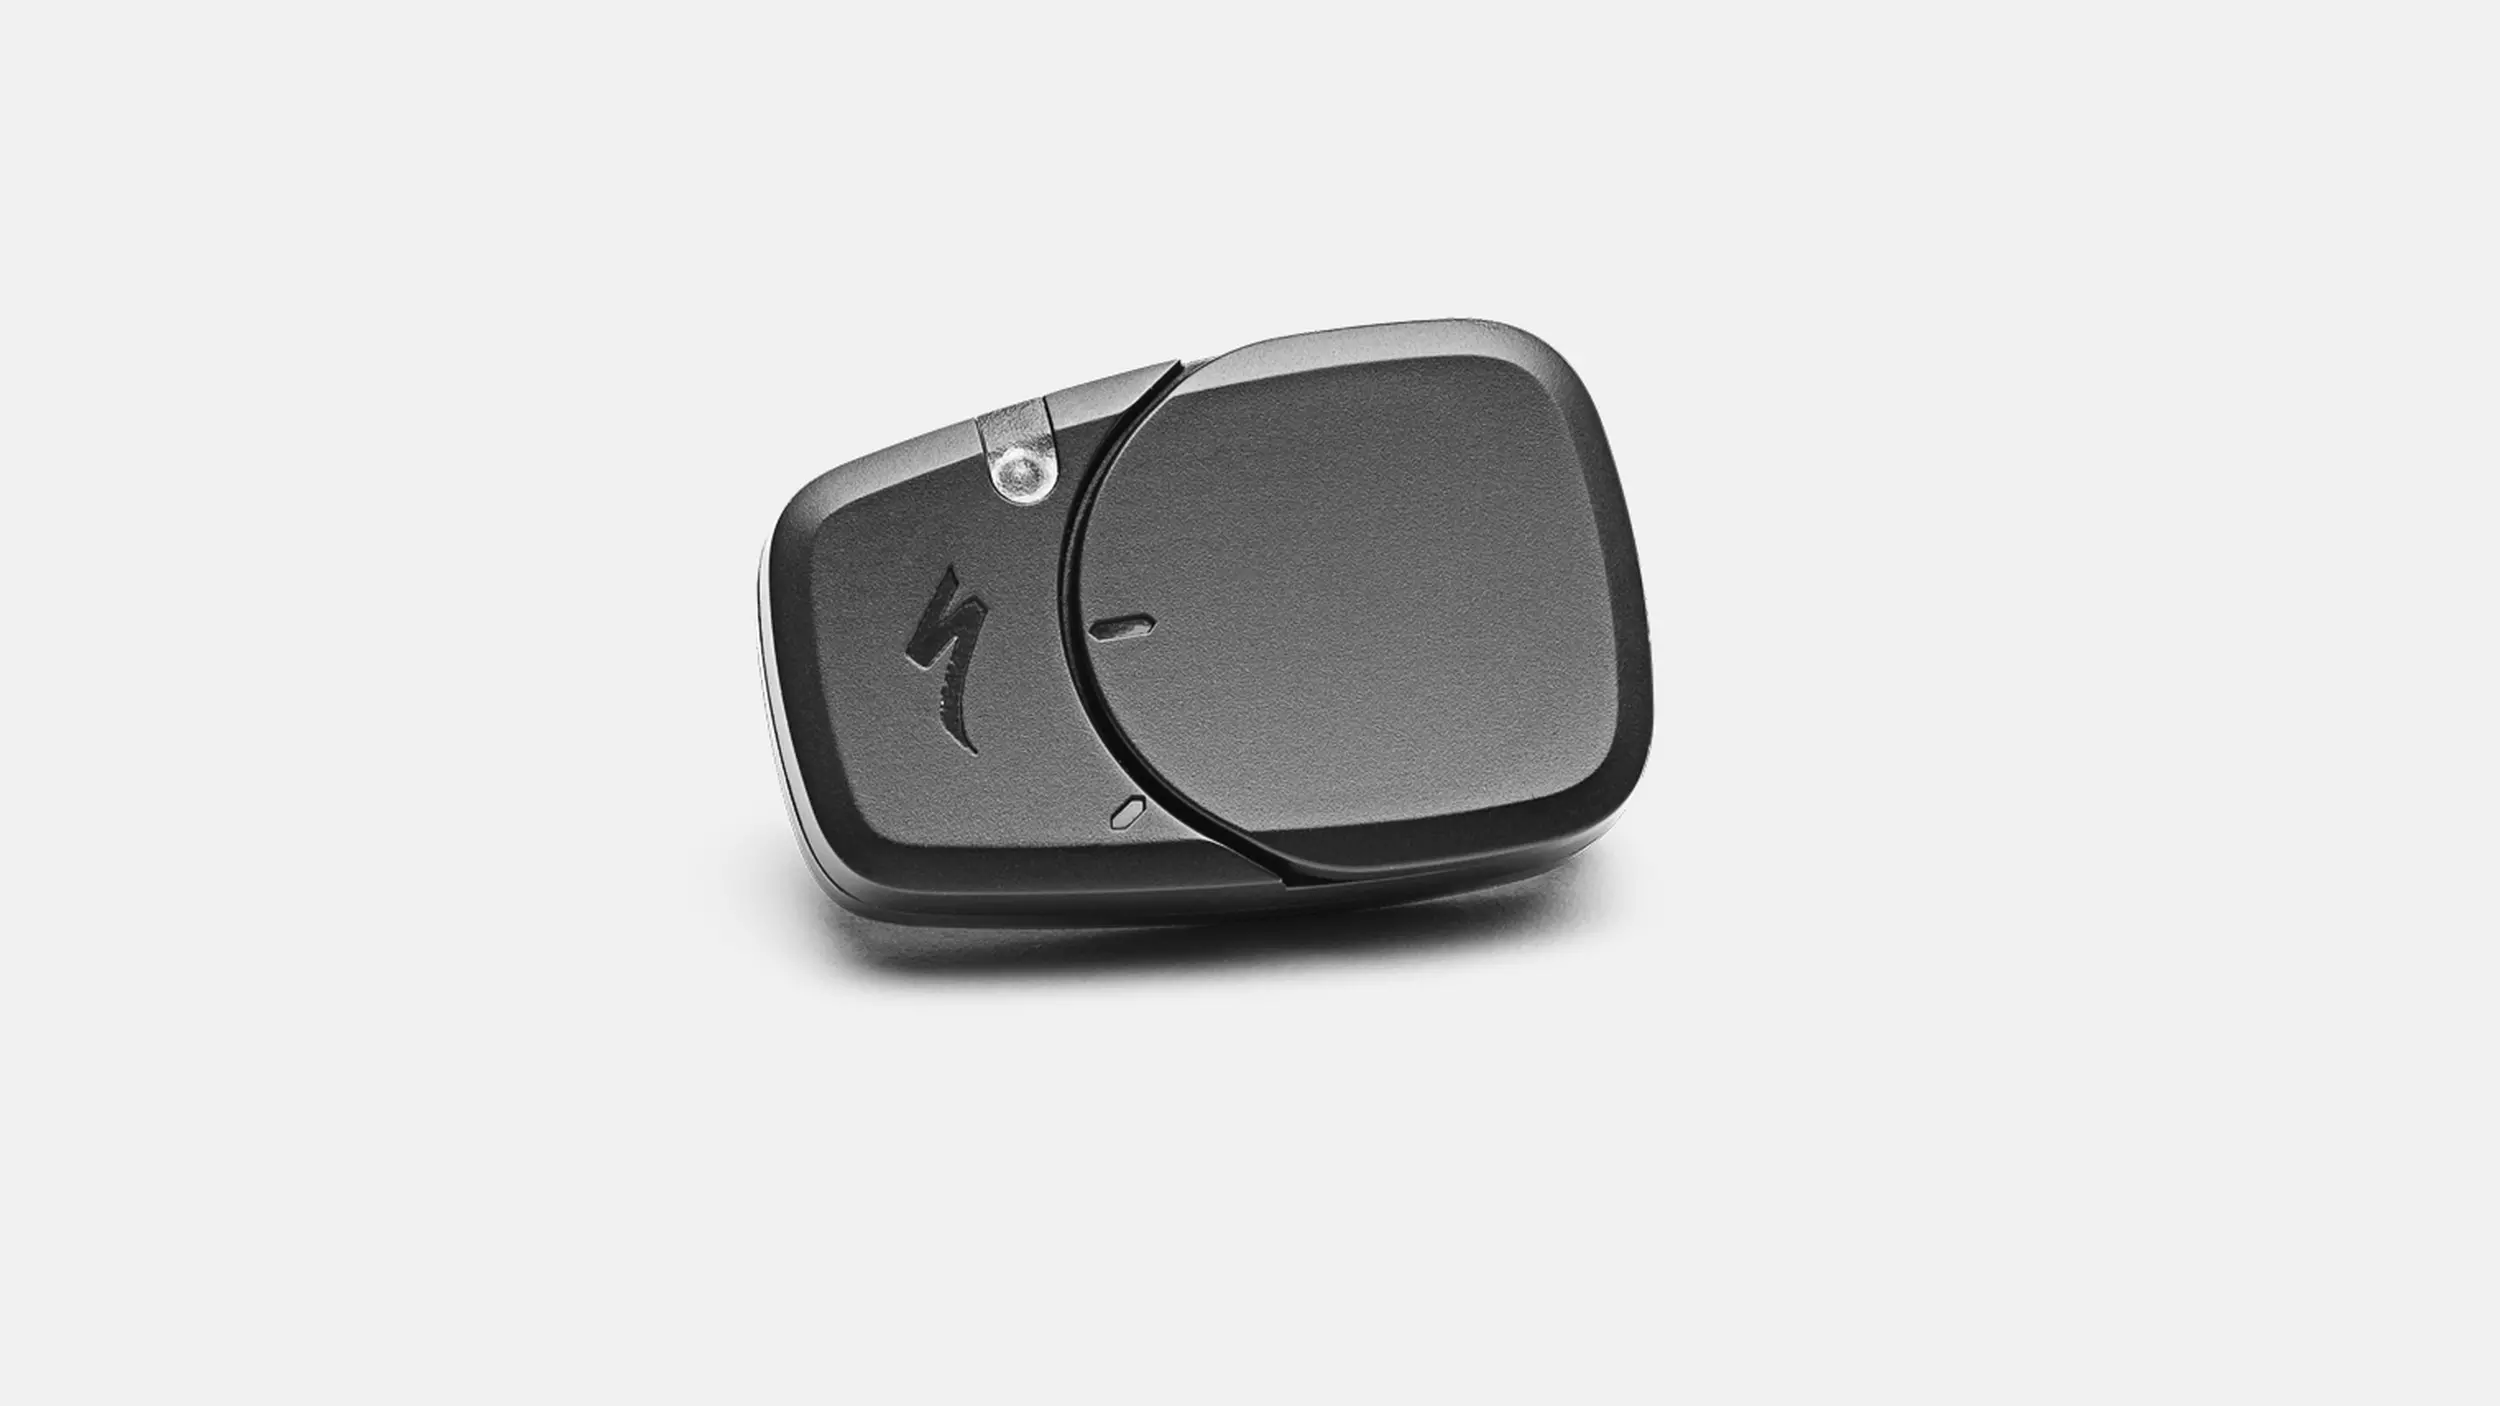
\includegraphics[width=7cm]{Graphics/angi.png}
\centering
\caption{Urządzenie ANGI, stworzone przez firmę Specialized.\cite{ANGI}}
\centering
\label{img:angi_img}
\end{figure}

%---------------------------------------------------------------------------















%\chapter{Pierwszy dokument}
\label{cha:pierwszyDokument}

W rozdziale tym przedstawiono podstawowe informacje dotyczące struktury prostych plików \LaTeX a. Omówiono również metody kompilacji plików z zastosowaniem programów \emph{latex} oraz \emph{pdflatex}.

%---------------------------------------------------------------------------

\section{Struktura dokumentu}
\label{sec:strukturaDokumentu}

Plik \LaTeX owy jest plikiem tekstowym, który oprócz tekstu zawiera polecenia formatujące ten tekst (analogicznie do języka HTML). Plik składa się z dwóch części:
\begin{enumerate}%[1)]
\item Preambuły -- określającej klasę dokumentu oraz zawierającej m.in. polecenia dołączającej dodatkowe pakiety;

\item Części głównej -- zawierającej zasadniczą treść dokumentu.
\end{enumerate}


\begin{lstlisting}
\documentclass[a4paper,12pt]{article}      % preambuła
\usepackage[polish]{babel}
\usepackage[utf8]{inputenc}
\usepackage[T1]{fontenc}
\usepackage{times}

\begin{document}                           % część główna

\section{Sztuczne życie}

% treść
% ąśężźćńłóĘŚĄŻŹĆŃÓŁ

\end{document}
\end{lstlisting}

Nie ma żadnych przeciwskazań do tworzenia dokumentów w~\LaTeX u w~języku polskim. Plik źródłowy jest zwykłym plikiem tekstowym i~do jego przygotowania można użyć dowolnego edytora tekstów, a~polskie znaki wprowadzać używając prawego klawisza \texttt{Alt}. Jeżeli po kompilacji dokumentu polskie znaki nie są wyświetlane poprawnie, to na 95\% źle określono sposób kodowania znaków (należy zmienić opcje wykorzystywanych pakietów).


%---------------------------------------------------------------------------

\section{Kompilacja}
\label{sec:kompilacja}


Załóżmy, że przygotowany przez nas dokument zapisany jest w pliku \texttt{test.tex}. Kolejno wykonane poniższe polecenia (pod warunkiem, że w pierwszym przypadku nie wykryto błędów i kompilacja zakończyła się sukcesem) pozwalają uzyskać nasz dokument w formacie pdf:
\begin{lstlisting}
latex test.tex
dvips test.dvi -o test.ps
ps2pdf test.ps
\end{lstlisting}
%
lub za pomocą PDF\LaTeX:
\begin{lstlisting}
pdflatex test.tex
\end{lstlisting}

Przy pierwszej kompilacji po zmiane tekstu, dodaniu nowych etykiet itp., \LaTeX~tworzy sobie spis rozdziałów, obrazków, tabel itp., a dopiero przy następnej kompilacji korzysta z tych informacji.

W pierwszym przypadku rysunki powinny być przygotowane w~formacie eps, a~w~drugim w~formacie pdf. Ponadto, jeżeli używamy polecenia \texttt{pdflatex test.tex} można wstawiać grafikę bitową (np. w formacie jpg).



%---------------------------------------------------------------------------

\section{Narzędzia}
\label{sec:narzedzia}


Do przygotowania pliku źródłowego może zostać wykorzystany dowolny edytor tekstowy. Niektóre edytory, np. GEdit, mają wbudowane moduły ułatwiające składanie tekstów w LaTeXu (kolorowanie składni, skrypty kompilacji, itp.).

Jednym z bardziej znanych środowisk do składania dokumentów  \LaTeX a jest {\em TeXstudio}, oferujące kompletne środowisko pracy. Zobacz: \url{http://www.texstudio.org}


Bardzo dobrym środowiskiem jest również edytor gEdit z wtyczką obsługującą \LaTeX a. Jest to standardowy edytor środowiska Gnome. Po instalacji wtyczki obsługującej \LaTeX~ zamienia się w wygodne i szybkie środowisko pracy.

\textbf{Dla testu łamania stron powtórzenia powyższego tekstu.}


Do przygotowania pliku źródłowego może zostać wykorzystany dowolny edytor tekstowy. Niektóre edytory, np. GEdit, mają wbudowane moduły ułatwiające składanie tekstów w LaTeXu (kolorowanie składni, skrypty kompilacji, itp.).
Jednym z bardziej znanych środowisk do składania dokumentów  \LaTeX a jest {\em TeXstudio}, oferujące kompletne środowisko pracy. Zobacz: \url{http://www.texstudio.org}
Bardzo dobrym środowiskiem jest również edytor gEdit z wtyczką obsługującą \LaTeX a. Jest to standardowy edytor środowiska Gnome. Po instalacji wtyczki obsługującej \LaTeX~ zamienia się w wygodne i szybkie środowisko pracy.
Po instalacji wtyczki obsługującej \LaTeX~ zamienia się w wygodne i szybkie środowisko pracy.

Do przygotowania pliku źródłowego może zostać wykorzystany dowolny edytor tekstowy. Niektóre edytory, np. GEdit, mają wbudowane moduły ułatwiające składanie tekstów w LaTeXu (kolorowanie składni, skrypty kompilacji, itp. itd. itp.).
Jednym z bardziej znanych środowisk do składania dokumentów  \LaTeX a jest {\em TeXstudio}, oferujące kompletne środowisko pracy. Zobacz: \url{http://www.texstudio.org}
Bardzo dobrym środowiskiem jest również edytor gEdit z wtyczką obsługującą \LaTeX a. Jest to standardowy edytor środowiska Gnome. Po instalacji wtyczki obsługującej \LaTeX~ zamienia się w wygodne i szybkie środowisko pracy.

Do przygotowania pliku źródłowego może zostać wykorzystany dowolny edytor tekstowy. Niektóre edytory, np. GEdit, mają wbudowane moduły ułatwiające składanie tekstów w LaTeXu (kolorowanie składni, skrypty kompilacji, itp.).
Jednym z bardziej znanych środowisk do składania dokumentów  \LaTeX a jest {\em TeXstudio}, oferujące kompletne środowisko pracy. Zobacz: \url{http://www.texstudio.org}
Bardzo dobrym środowiskiem jest również edytor gEdit z wtyczką obsługującą \LaTeX a. Jest to standardowy edytor środowiska Gnome. Po instalacji wtyczki obsługującej \LaTeX~ zamienia się w wygodne i szybkie środowisko pracy.

%---------------------------------------------------------------------------

\section{Przygotowanie dokumentu}
\label{sec:przygotowanieDokumentu}

Plik źródłowy \LaTeX a jest zwykłym plikiem tekstowym. Przygotowując plik
źródłowy warto wiedzieć o kilku szczegółach:

\begin{itemize}
\item
Poszczególne słowa oddzielamy spacjami, przy czym ilość spacji nie ma znaczenia.
Po kompilacji wielokrotne spacje i tak będą wyglądały jak pojedyncza spacja.
Aby uzyskać {\em twardą spację}, zamiast znaku spacji należy użyć znaku {\em
tyldy}.

\item
Znakiem końca akapitu jest pusta linia (ilość pusty linii nie ma znaczenia), a
nie znaki przejścia do nowej linii.

\item
\LaTeX~sam formatuje tekst. \textbf{Nie starajmy się go poprawiać}, chyba, że
naprawdę wiemy co robimy.
\end{itemize} 



%\chapter{Testy}

\section{Test URL-a}

Wejdź na stronę \url{https://www.google.pl/} i wpisz szukane zdanie.

\clearpage

\section{Test dzielenia wdów}

Lorem ipsum dolor sit amet, ex est alia dolorem commune. Duo modo errem no. Ea harum doming atomorum mei. Consul animal malorum cu qui, sumo dicta graece an est, vim ei clita regione.

Vel eu quando doming fastidii, mei graeco indoctum an, legere theophrastus in pro. Te mei probatus eleifend interpretaris. Est no autem liber vituperatoribus, cu mea dicam constituto. Ea laudem tritani consectetuer sit, sanctus patrioque expetendis vix in. Duo id fugit adversarium signiferumque, an quot modus molestiae qui.

Ut paulo definiebas pro. Mea an quod esse. Et atomorum facilisis moderatius sit. Graeco iudicabit forensibus in vel. Eam cu lorem aeterno offendit, cu vix nulla congue posidonium. Vel lucilius evertitur vituperata no.

Mea eu graecis prodesset. Et tota eius nec. Ei etiam oratio has, vel ei homero eripuit invenire. Sed ex errem intellegebat, sea et elitr intellegat constituto. Nostro voluptua accusamus eos in, ei sale admodum has. Vim ne consetetur reformidans, ad has malis recusabo persequeris, per etiam virtute invenire in.

Te nihil eruditi eam, sit aperiam accusam mediocritatem at. Nec ne nonumy dictas disputationi, vis ridens sadipscing ex. Harum euripidis ex vix, at consetetur instructior signiferumque mel, at mei elitr honestatis. Id sit congue vituperata. Temporibus eloquentiam no eum.

Pro id esse phaedrum, nostro iudicabit eos ut. Sit ea aperiam alienum, harum audiam voluptua cu usu. Iudico invenire te vel, id suscipit disputando pri. Ut sumo expetenda mea.

Cum at idque nullam aperiam, vis ex aeque ponderum luptatum. Vix soluta graeco dissentiet ut, ut est reque periculis similique, ut dicta dicant repudiare sea. Ne dolor legendos signiferumque ius, at eirmod convenire qui. Suas numquam conceptam mei ex. Autem homero eos et, sea dicta alienum iudicabit ut.

Ea duo consulatu vulputate, id elit perpetua cum. His ei aeque saepe audiam. Prompta laoreet facilisi ne sed, per hinc consetetur te, oratio fuisset ullamcorper mel at. Quis suscipiantur ne nec, agam efficiendi usu in.

Vis eu iuvaret singulis appellantur, usu ex saepe omittantur. Sed possit mnesarchum at, usu illum choro oratio in, et debet dolor vix. Mel aperiri suscipiantur ne, te per illum fuisset, lorem pericula mei ad. Pri id tale lucilius dissentiet, id sea sonet expetenda. Agam sensibus persequeris sed no, eum at tamquam sanctus.

Omnis exerci soleat ut vis. Rebum vidisse sea ex. Ius animal gubergren efficiantur ad, mollis probatus nec ut. Meis platonem ex vel, ut qui tale tritani equidem. Vide meis fuisset mel at, nam an assum delenit gubergren. No illum reprimique vim, te augue nullam per, ludus dicant suscipiantur ne sed.

An pri mediocrem deseruisse, ad sumo audire dissentiet sit. Sit ea civibus lobortis. Etiam ceteros commune ei vis. Pro ei equidem vivendo. Quo ne prima periculis omittantur, ex rebum veritus sit, ei dolor maiestatis mea.

\subsection{Lorem ipsum}

Et mel munere quodsi sapientem. Essent legimus ne pro. Est ornatus definiebas et. No habemus docendi ius, purto sapientem mei at. Tamquam vivendo necessitatibus has at, no habemus praesent nec. No quo modus iudicabit scriptorem. Modus intellegebat ea vim. Cu ius lorem regione offendit, ne accusata sensibus vituperatoribus quo. Sit ut iuvaret indoctum. Ut mea sale justo. Sapientem definitionem ius eu, at sea quem doming. Facete conclusionemque ut nec, vix at duis eius. Eos quot consequuntur et, ornatus liberavisse ne mei.

Per an dicam commodo tractatos, usu in timeam numquam tacimates. Case delectus eu sea, usu audiam eleifend tincidunt id, nec at decore discere mentitum. Ut elit veri eloquentiam his, ceteros tractatos ea has. Duo impetus scribentur et, eu quo errem everti, ad recusabo consulatu ius. Fastidii comprehensam pri ea, ex duo augue quando denique. Eos aeterno deserunt sententiae cu, ius quas tation patrioque ex.

Id autem scripta explicari nec, congue quidam possit te sit. Et usu ipsum bonorum graecis, ferri verear deterruisset eum cu. Purto porro accommodare cu vim. Cum ei tritani pertinacia voluptaria.



% itd.
% \appendix
% \include{dodatekA}
% \include{dodatekB}
% itd.

\printbibliography

\end{document}